\documentclass{article}
\usepackage{tikz}
\begin{document}

\section{Binary search tree}

After inserting 50, 30, 70, 20, 40, 60 and 80 the tree looks like this:

\begin{center}
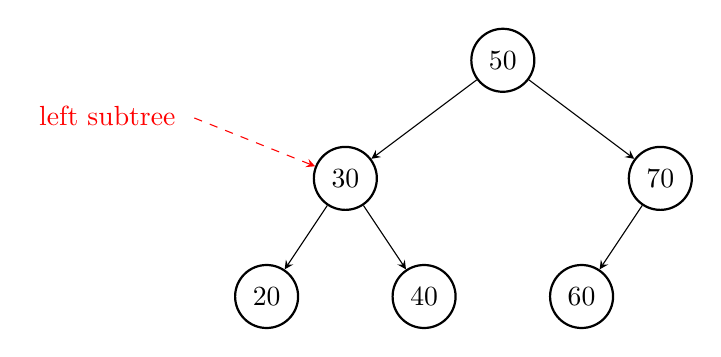
\begin{tikzpicture}[
  every node/.style={circle, draw, thick, minimum size=8mm},
  level/.style={sibling distance=40mm/#1},
  level distance=15mm,
  ->, >=stealth
]
\node (root) {50}
  child {node (a) {30}
    child {node {20}}
    child {node {40}}
  }
  child {node (b) {70}
    child {node {60}}
    child[missing]
  };
\draw[red, dashed, <-] (a) -- ++(-2,0.8) node[draw=none, left] {left subtree};
\end{tikzpicture}
\end{center}

\end{document}
